\Needspace{20\baselineskip}
\section{性能分析与 GPU 硬件}
\label{l14:sec:hardware}

\subsection{性能数据所回答的问题}

\term{性能分析}{profiling}是在程序实际执行时，收集运行时间、事件时间线和硬件计数器，再把这些观察与源代码联系起来的过程。\term{性能分析器}{profiler}可以观察处理器何时工作、数据经过哪些存储层级、指令为何等待，以及哪些代码占用了主要执行时间。程序的数学表达式给出了要完成的运算；执行性能还取决于线程组织、访存布局、资源分配和具体硬件。

优化需要先建立正确的程序，再测量其开销，并针对主要限制修改实现。每次修改之后都要重新检查结果和运行时间，因为减少一种开销可能增加另一种开销。例如，共享内存分块能减少重复的全局读取，同时也会引入共享读取、块内同步和片上资源占用；这些成本共同决定最终收益。

分析尺度可以分为应用和内核两层。应用层关心主机准备数据、设备传输、内核计算与同步之间的时间关系；内核层关心某次内核执行期间的指令发射、计算流水线、缓存及存储系统。系统级分析工具（Nsight Systems）适合先定位应用中的主要耗时区间，内核级分析工具（Nsight Compute）再用于解释目标内核内部的硬件行为。一次内核执行变快以后，还应回到应用层确认总时间是否下降。

设目标内核原先占应用总时间的比例为 $f$，对它的加速比为 $s$，其余部分的时间保持不变。将原总时间归一化为 $1$，优化后的时间为 $(1-f)+f/s$，所以应用加速比为
\begin{equation}
  S_{\mathrm{app}}=\frac{1}{(1-f)+f/s}.
  \label{l14:eq:amdahl}
\end{equation}
例如，某内核只占总时间的 $20\%$，即使它达到 $4$ 倍加速，应用也只有 $1/(0.8+0.2/4)\approx1.18$ 倍加速。这个关系说明了为什么应先确定耗时位置，再选择值得深入分析的内核。

\subsection{线程组织与硬件执行层级}

在统一计算设备架构（CUDA）的执行模型中，一次内核启动产生一个\term{网格}{grid}，网格由\term{线程块}{thread block}组成，线程块内包含线程。GPU 的主要通用执行单元是\term{流式多处理器}{streaming multiprocessor，SM}。一个普通线程块的线程在同一个 SM 上执行，因此能够通过该 SM 的共享内存交换数据并进行块内同步；一个 SM 在资源允许时可以同时驻留多个线程块。

线程块内部以 $32$ 个线程组成一个\term{线程束}{warp}。线程束中的线程共享指令发射过程，各线程仍保留自己的寄存器状态和数据索引。调度器从驻留线程束中选择已经具备执行条件的线程束，并向相应流水线发射指令。于是，线程束等待某次访存时，调度器可以发射其他就绪线程束的指令，这构成了\term{延迟隐藏}{latency hiding}的基础。

一个 SM 通常进一步划分为若干子分区（SM subpartition，SMSP），其中包含线程束调度器、寄存器资源和执行流水线。芯片级还可能采用图形处理簇（graphics processing cluster，GPC）、纹理处理簇（texture processing cluster，TPC）等组织层级。这些结构帮助解释硬件图，但程序中的线程块与这些簇没有固定的一一对应关系。线程块到 SM 的分配、每个 SM 可驻留的线程束数，以及每周期能够发射的指令，都要结合所分析的 GPU 判断。

不同指令会使用不同执行资源：普通浮点乘加使用浮点流水线，地址计算通常需要整数指令，读取与写入使用加载／存储流水线，某些数学函数使用特殊函数单元（special function unit，SFU）。张量核心（Tensor Core）承担特定矩阵运算。一个内核是否有效利用硬件，必须对应到它实际执行的指令类别；某种流水线很忙，无法直接推出全部计算资源都达到了峰值。

\begin{keybox}[title={并行数量与执行能力}]
驻留线程束提供可供调度的工作，就绪线程束提供当前可发射的工作，执行流水线决定当前能接收什么指令。这三个层次共同限制吞吐率。增加线程数只有在改善其中的实际限制时才会带来收益。
\end{keybox}

\subsection{存储空间、物理位置与缓存路径}

CUDA 的存储空间规定数据的可见范围和访问方式；物理存储层级决定数据放在哪里、如何被缓存，以及访问经过哪些硬件。理解性能指标时，需要同时掌握这两种含义。表\ref{l14:tab:memory-spaces}给出与本讲相关的对应关系。

\begin{table}[htbp]
\centering\small
\caption{存储空间与典型硬件实现}
\label{l14:tab:memory-spaces}
\begin{tabularx}{\textwidth}{@{}>{\raggedright\arraybackslash}p{27mm}YY@{}}
\toprule
存储空间 & 典型物理位置或访问路径 & 分析时的关注点\\
\midrule
全局内存 & 设备内存，通常经过 L2 与 L1／纹理缓存路径 & 访问合并、缓存复用和各层实际流量\\
共享内存 & SM 上显式管理的片上存储 & 线程块内复用、存储体冲突和读取指令压力\\
常量内存 & 设备内存及相应常量缓存路径 & 同一线程束访问相同地址时的广播\\
纹理／表面内存 & 设备内存及纹理相关缓存路径 & 专用访问方式及局部性\\
局部内存 & 线程私有地址空间，数据可能位于设备内存并经过缓存 & 大型私有数组和寄存器溢出带来的访存\\
寄存器 & SM 的寄存器文件；按线程保存状态，并受分配粒度约束 & 寄存器用量、依赖链和可驻留线程束数\\
\bottomrule
\end{tabularx}
\end{table}

一级缓存（L1 cache）靠近 SM，二级缓存（L2 cache）位于更外层并由多个 SM 共享。许多架构让 L1 与共享内存共用一部分物理片上容量，但两者的管理方式不同：共享内存由程序显式写入、读取和同步，L1 则依照缓存机制自动保存访问过的数据。共享内存容量的配置可能影响可用缓存容量，也可能限制同时驻留的线程块数。

\term{局部内存}{local memory}中的“局部”表示线程私有的可见性。它不能作为低延迟片上存储的保证。当编译器无法把某些线程私有变量保留在寄存器中时，这些变量可能被放到局部内存，从而增加实际加载和存储。寄存器数量因此存在两方面作用：更多寄存器可以保存更多可复用数据和独立累加器，但每线程用量过高又可能压低占用率，甚至导致\term{寄存器溢出}{register spilling}。

\term{缓存命中}{cache hit}表示所需数据已经位于当前检查的缓存层；\term{缓存未命中}{cache miss}则需要继续向下一级请求数据。\term{时间局部性}{temporal locality}来自一段时间内反复访问同一数据，\term{空间局部性}{spatial locality}来自访问相邻地址。缓存容量有限，旧数据会因替换而被移出，因此同一个全局地址的多次访问不一定每次都需要访问设备内存，也不一定一直能够命中同一层缓存。

把一次加载简单理解为“L1 未命中后读取 L2，L2 未命中后读取设备内存”，能够解释数据来源；要进一步理解吞吐率，还必须考虑请求队列、地址标签检查、数据返回和执行依赖。图\ref{l14:fig:l1-path}展示了这种更具体的路径。共享请求与全局请求可以经过相关的入口和数据通路，因此即使设备内存流量不大，片上请求处理也可能形成限制。

\begin{figure}[htbp]
\centering
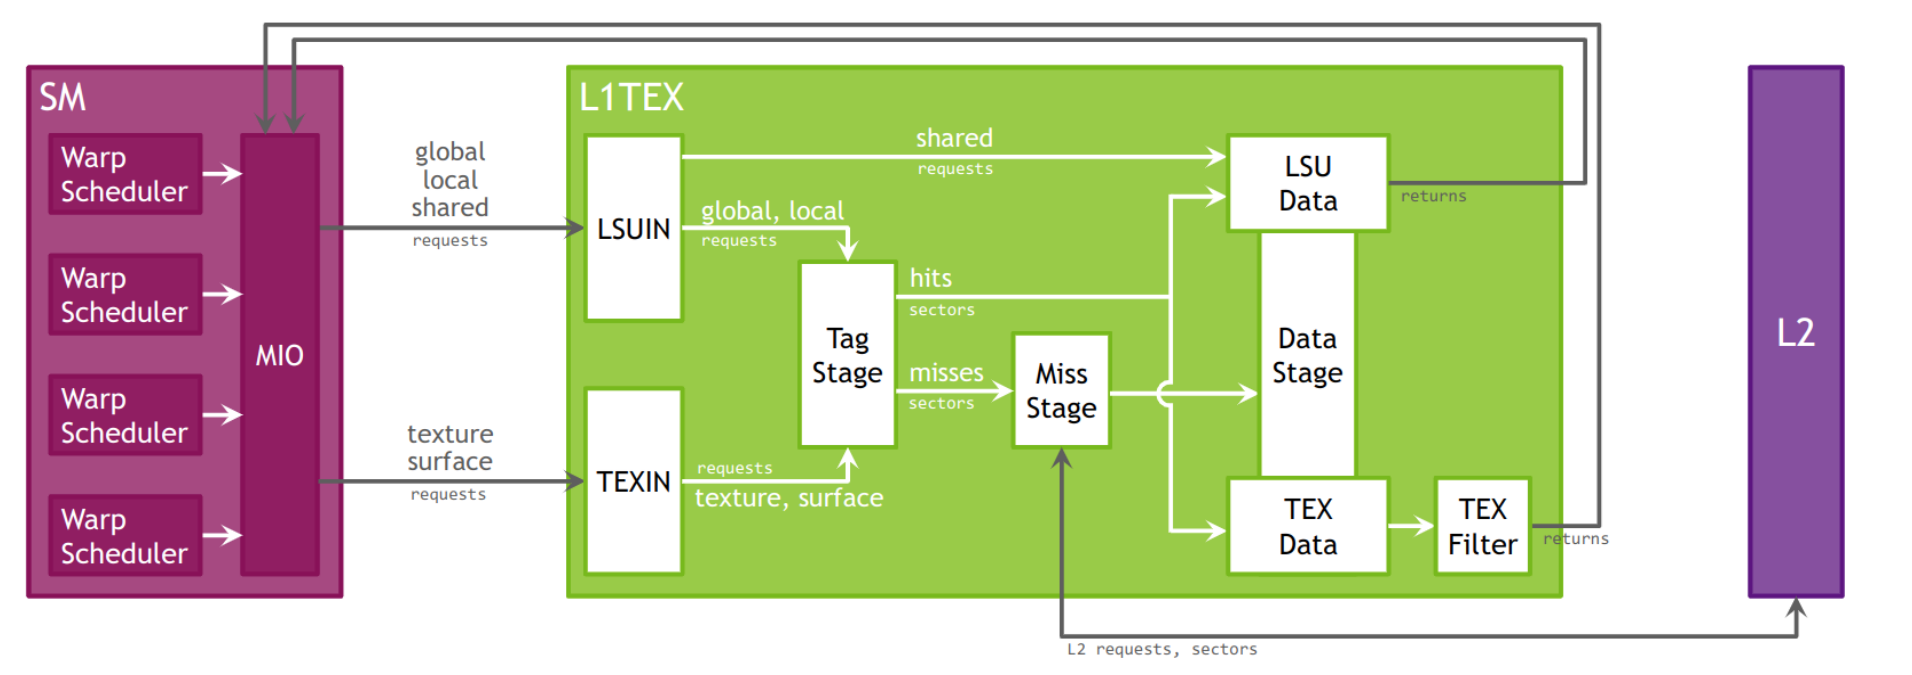
\includegraphics[width=\textwidth]{l1_path.png}
\caption{线程束调度器到 L1／纹理单元及 L2 的请求与返回路径。共享访问需要经过片上的请求处理和数据通路；全局访问还涉及缓存标签检查与未命中处理。}
\label{l14:fig:l1-path}
\end{figure}

这些层级还解释了为何同一份 CUDA 代码在不同 GPU 上呈现不同的瓶颈。缓存容量、每个 SM 的执行资源、可驻留线程束数和设备内存带宽都可能改变。比较硬件时，应保留问题规模、数据类型、编译选项和计时范围，再依据对应设备的计数器解释差异。
